\documentclass{article}
\usepackage{polski}
\usepackage[utf8]{inputenc}
\usepackage{graphicx} 
\title{Dokumentacja projektu z Programowania Sieciowego}
\date{\today}
\author{Karol Błędziński, Kamil Gorzała, Jakub Kołomański}

\begin{document}


 \maketitle
 \newpage
 \newpage
 \section{Model TCP/IP}
\subsection{Opis}
	Model TCP/IP (ang. Transmission Control Protocol/Internet Protocol) – teoretyczny model warstwowej struktury protokołów komunikacyjnych. Model TCP/IP został stworzony w latach 70. XX wieku w DARPA, aby pomóc w tworzeniu odpornych na atak sieci komputerowych. Potem stał się podstawą struktury Internetu.
	
Podstawowym założeniem modelu TCP/IP jest podział całego zagadnienia komunikacji sieciowej na szereg współpracujących ze sobą warstw (ang. layers). Każda z nich może być tworzona przez programistów zupełnie niezależnie, jeżeli narzucimy pewne protokoły według których wymieniają się one informacjami. Założenia modelu TCP/IP są pod względem organizacji warstw zbliżone do modelu OSI. Jednak liczba warstw jest mniejsza i bardziej odzwierciedla prawdziwą strukturę Internetu. Model TCP/IP składa się z czterech warstw.

Każdy protokół sieciowy można przyporządkować do określonej warstwy modelu TCP/IP. Pewną szczególną cechą rodziny protokołów TCP/IP używanej w Internecie jest podział protokołów z warstwy aplikacyjnej i połączeniowej. Niektóre protokoły z warstwy aplikacji wykorzystują tylko pewne protokoły z warstwy transportowej.

Protokoły DNS, NTP wykorzystują tylko protokół UDP z warstwy transportowej. Protokoły FTP, SMTP, POP3, SSH, IRC posługują się tylko TCP. Natomiast SMB używa obu protokołów.

Protokół SSL ma szczególną rolę. Może zostać umieszczony pomiędzy każdym połączeniowym protokołem warstwy aplikacji a TCP. Dzięki jego wykorzystaniu dane przesyłane przez aplikacje mogą zostać zaszyfrowane.

Niektóre protokoły z warstwy aplikacji, jak np. SMB nie działają zwykle w Internecie. Są wykorzystane w sieciach lokalnych do udostępniania usług, jak np. zdalne drukarki czy dyski.

W systemie GNU/Linux oraz innych odpowiednikach Uniksa dokładną listę protokołów transportowych można znaleźć w pliku.

W dzisiejszych czasach, praktycznie każdy system operacyjny posiada domyślnie zainstalowane protokoły TCP/IP.

Istnieje także Lightweight TCP/IP, szerzej znany jako darmowy stos TCP/IP dla systemów wbudowanych, czyli będących integralną częścią obsługiwanego przez nie sprzętu - jest to stos protokołów dla systemów obsługujących zarówno amatorskie jak i zaawansowane urządzenia, często budowane z wykorzystaniem programowalnych układów FPGA (np. sprzętowe serwery WWW, FTP). Istnieją także proste stosy TCP/IP realizowane całkowicie sprzętowo.
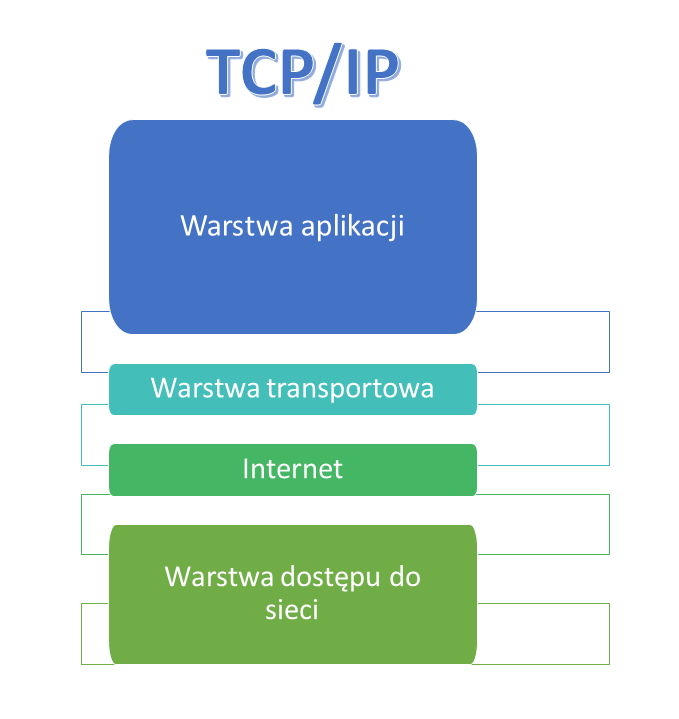
\includegraphics[width=0.7\textwidth]{tcp.png}

\section{Model ISO/OSI}
\subsection{Opis}
	Model OSI (pełna nazwa ISO OSI RM, ang. ISO Open Systems Interconnection Reference Model – model odniesienia łączenia systemów otwartych) lub OSI – standard zdefiniowany przez ISO oraz ITU-T opisujący strukturę komunikacji sieciowej.

Międzynarodowa Organizacja Normalizacyjna (ang. International Organization for Standardization) na początku lat osiemdziesiątych dostrzegła potrzebę stworzenia modelu sieciowego, dzięki któremu producenci mogliby opracowywać współpracujące ze sobą rozwiązania sieciowe. W taki sposób powstała specyfikacja Open Systems Interconnection Reference Model, która do polskich norm została zaadaptowana w 1995 roku.

Model ISO OSI RM jest traktowany jako model odniesienia (wzorzec) dla większości rodzin protokołów komunikacyjnych. Podstawowym założeniem modelu jest podział systemów sieciowych na 7 warstw (ang. layers) współpracujących ze sobą w ściśle określony sposób. Został przyjęty przez ISO w 1984 roku a najbardziej interesującym organem jest wspólny komitet powołany przez ISO/IEC, zwany Joint Technical Committee 1- Information Technology (JTC1). Formalnie dzieli się jeszcze na podkomitety SC.
 
 Model OSI definiuje jakie zadania oraz rodzaje danych mogą być przesyłane między warstwami w całkowitym oderwaniu od ich fizycznej i algorytmicznej realizacji, czyli zakłada istnienie warstw abstrakcji w medium transmisyjnym, sprzęcie oraz oprogramowaniu i wokół tych warstw orientuje specyficzne dla nich protokoły, realizowane przez te protokoły usługi świadczone wyższym warstwom oraz posiadane interfejsy, umożliwiające dostęp do warstwy przez procesy z innych warstw. Mimo iż każda z warstw sama nie jest funkcjonalna, to możliwe jest projektowanie warstwy w całkowitym oderwaniu od pozostałych. Jest to realne, jeżeli wcześniej zdefiniuje się protokoły wymiany danych pomiędzy poszczególnymi warstwami.
 
 W praktyce Model OSI został częściowo zmodyfikowany. Najczęstszą zmianą było połączenie warstwy fizycznej oraz łącza danych w jedną. Wynikało to z praktycznych cech tych warstw, które powodowały, że nie dało się odseparować ich pracy od siebie. Nie należy mylić Modelu OSI-RM z TCP/IP. Mimo pewnego podobieństwa oba te modele nie są w pełni zgodne.
 


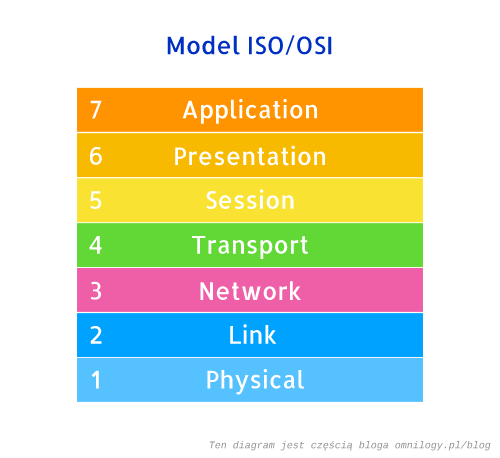
\includegraphics[width=0.6\textwidth]{OSI.png}

\newpage

\section{SDN}
\subsection{Opis}
	Technologia definiowana przez oprogramowanie (SDN) to podejście do przetwarzania w chmurze, które ułatwia zarządzanie siecią i umożliwia programowo wydajną konfigurację sieci w celu poprawy wydajności i monitorowania sieci.  SDN ma na celu zajęcie się faktem, że architektura statyczna tradycyjnych sieci jest zdecentralizowana i złożona, podczas gdy obecne sieci wymagają większej elastyczności i łatwiejszego rozwiązywania problemów. SDN sugeruje scentralizować inteligencję sieciową w jednym komponencie sieciowym poprzez odłączenie procesu przekazywania pakietów sieciowych (płaszczyzny danych) od procesu routingu (płaszczyzny kontrolnej). Płaszczyzna kontrolna składa się z jednego lub więcej kontrolerów, które są uważane za mózg sieci SDN, w której włączona jest cała inteligencja. Jednak centralizacja danych wywiadowczych ma swoje wady, jeśli chodzi o bezpieczeństwo,  skalowalność i elastyczność  i jest to główny problem SDN.

SDN był powszechnie kojarzony z protokołem OpenFlow (do zdalnej komunikacji z elementami płaszczyzny sieci w celu określenia ścieżki pakietów sieciowych przez przełączniki sieciowe) od czasu jego pojawienia się w 2011 roku. Jednak od 2012 roku  OpenFlow dla wielu firmy nie są już wyłącznym rozwiązaniem, dodały własne techniki. Należą do nich Open Network Environment firmy Cisco Systems i platforma wirtualizacji sieci firmy Nicira.

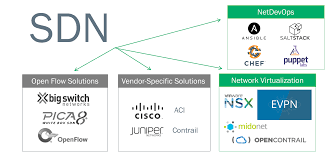
\includegraphics[width=0.9\textwidth]{sdn.png}
 \newpage
\section{APIC-EM}
\subsection{Opis}
	APIC EM rozszerza infrastrukturę Application Centric (ACI) na sieć WAN i dostęp. ACI zapewnia scentralizowaną automatyzację profilów aplikacji opartych na regułach. Dzięki programowalności zautomatyzowana kontrola sieci pomaga działom IT szybko reagować na nowe możliwości biznesowe. APIC EM można pobrać bez dodatkowych opłat, korzystając z bezpłatnego członkostwa w społeczności Cisco DevNet.

Funkcje i możliwości

APIC EM i jego aplikacje są częścią portfolio Cisco ONE Software. Kontroler zapewnia nisko-ryzykowne, stopniowe podejście do wdrażania technologii sieciowej definiowanej programowo (SDN) w środowiskach branżowych i kampusowych. Dzięki podejściu zorientowanemu na aplikację kontroler automatyzuje dostarczanie kompleksowej infrastruktury w celu szybkiego wdrażania aplikacji i usług.

funkcje

Oprogramowanie działające na dowolnym serwerze x86, oferowane jako oprogramowanie lub urządzenie
Zaawansowany GUI bez umiejętności programowania
Zintegrowana analityka, polityka i abstrakcja sieci
Korzyści

Masowo uproszczona konfiguracja i udostępnianie

Kontroler automatyzuje wdrażanie i sprawdzanie zgodności polityk sieciowych w całej sieci end-to-end.

Ochrona inwestycji

Kontroler działa z istniejącą infrastrukturą sieci. Nie ma potrzeby przeprowadzania wymiany infrastruktury. Nie jest potrzebny żaden nowy sprzęt sieciowy.

Otwartość, programowalność i personalizacja

APIC EM jest wysoce programowalny poprzez otwarte interfejsy API (transfer danych reprezentacyjnych [RESTful] i OSGi). Umożliwia niezależnym twórcom oprogramowania tworzenie innowacyjnych usług sieciowych i aplikacji, które przyczyniają się do wzrostu gospodarczego.

Polityka biznesowa do konfiguracji sieci

Sterownik automatycznie tłumaczy zasady biznesowe na strategie na poziomie urządzeń sieciowych i umożliwia egzekwowanie zasad w sieciach typu end-to-end.
\newpage
\section{Python}
\subsection{Opis}
	Python jest interpretowanym, interaktywnym językiem programowania stworzonym przez Guido van Rossuma w 1990 roku. Posiada w pełni dynamiczny system typów i automatyczne zarządzanie pamięcią, jest zatem podobny do takich języków, jak Tcl, Perl, Scheme czy Ruby. Python rozwijany jest jako projekt Open Source, zarządzany przez niedochodową Python Software Fundation.
	

\includegraphics[width=0.9\textwidth]{python.png}
\subsection{Rozwój języka}
	Pythona stworzył we wczesnych latach 90. Guido van Rossum – jako następcę języka ABC, stworzonego w Centrum voor Wiskunde en Informatica (CWI – Centrum Matematyki i Informatyki w Amsterdamie). Van Rossum jest głównym twórcą Pythona, choć spory wkład w jego rozwój pochodzi od innych osób. Z racji kluczowej roli, jaką van Rossum pełni przy podejmowaniu ważnych decyzji projektowych, często określa się go przydomkiem „Benevolent Dictator for Life” (BDFL).

Nazwa języka nie pochodzi od zwierzęcia lecz od serialu komediowego emitowanego w latach siedemdziesiątych przez BBC – „Monty Python’s Flying Circus” (Latający cyrk Monty Pythona). Projektant, będąc fanem serialu i poszukując nazwy krótkiej, unikalnej i nieco tajemniczej, uznał tę za świetną.

Wersja 1.2 była ostatnią wydaną przez CWI. Od 1995 roku Van Rossum kontynuował pracę nad Pythonem w Corporation for National Research Initiatives (CNRI) w Reston w Wirginii, gdzie wydał kilka wersji Pythona, do 1.6 włącznie. W 2000 roku van Rossum i zespół pracujący nad rozwojem jądra Pythona przenieśli się do BeOpen.com by założyć zespół BeOpen PythonLabs. Pierwszą i jedyną wersją wydaną przez BeOpen.com był Python 2.0.

Po wydaniu wersji 1.6 i opuszczeniu CNRI przez van Rossuma, który zajął się programowaniem komercyjnym, uznano za wysoce pożądane, by Pythona można było używać z oprogramowaniem dostępnym na licencji GPL. CNRI i Free Software Foundation (FSF) podjęły wspólny wysiłek w celu odpowiedniej modyfikacji licencji Pythona. Wersja 1.6.1 była zasadniczo identyczna z wersją 1.6, z wyjątkiem kilku drobnych poprawek oraz licencji, dzięki której późniejsze wersje mogły być zgodne z licencją GPL. Python 2.1 pochodzi zarówno od wersji 1.6.1, jak i 2.0.

Po wydaniu Pythona 2.0 przez BeOpen.com Guido van Rossum i inni programiści z PythonLabs przeszli do Digital Creations. Cała własność intelektualna dodana od tego momentu, począwszy od Pythona 2.1 (wraz z wersjami alpha i beta), jest własnością Python Software Foundation (PSF), niedochodowej organizacji wzorowanej na Apache Software Foundation.
 \subsection{Filozofia Pythona} 
 Python realizuje jednocześnie kilka paradygmatów. Podobnie do C++, a w przeciwieństwie do Smalltalka nie wymusza jednego stylu programowania, pozwalając na stosowanie różnych. W Pythonie możliwe jest programowanie obiektowe, programowanie strukturalne i programowanie funkcyjne. Typy sprawdzane są dynamicznie, a do zarządzania pamięcią stosuje się garbage collection.

Choć w jego popularyzacji kładzie się nacisk na różnice w stosunku do Perla, Python jest pod wieloma względami do niego podobny. Jednakże projektanci Pythona odrzucili złożoną składnię Perla na rzecz bardziej oszczędnej i – ich zdaniem – bardziej czytelnej. Mimo że podobnie do Perla, Python jest czasem klasyfikowany jako język skryptowy, wykorzystuje się go do tworzenia dużych projektów jak serwer aplikacji Zope, system wymiany plików Mojo Nation czy nawet oprogramowanie klasy ERP – OpenERP.
 \newpage
\section{jupyter}
\subsection{Opis}
Jupter to w pierwszej kolejności przeglądarkowe środowisko do pisania skryptów. Pierwotnym projektem na bazie którego powstał Jupyter jest IPYTHON, którego ostatnim wydaniem jako osobnego programu była wersja 3.0. Od wersji 4.0 IPython funkcjonuje już jako podstawowy kernel Jupytera, o czym przeczytamy dalej.

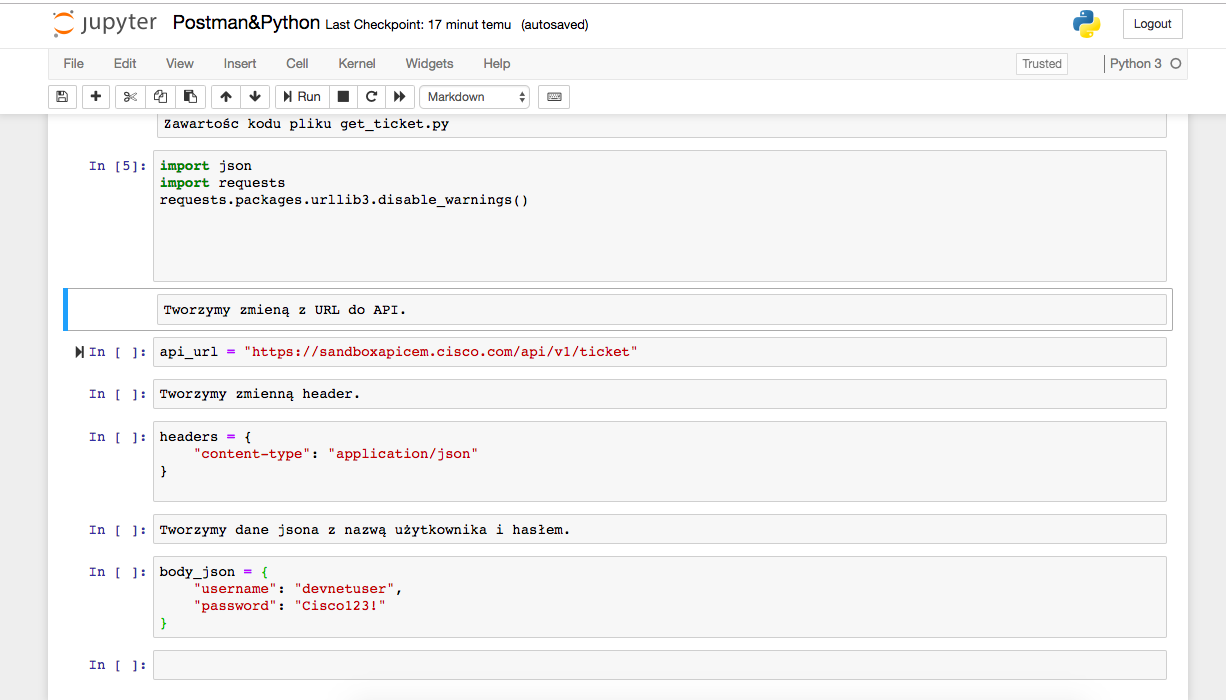
\includegraphics[width=1\textwidth]{jupyter.png}
{Przykładowe użycie jupytera w projekcie z Postman.}
\subsection{Markdown}
Komórki notesowe mają swoje typy. Domyślnym typem jest oczywiście komórka na wpisanie kodu. Drugim ciekawym typem jest komórka interpretująca MARKDOWN. Dzięki temu w Jupyterze można ładnie komentować kod, jak także obiekty wynikowe.
\newpage
\section{GIT}
\subsection{Opis}
Rozproszony system kontroli wersji. Stworzył go Linus Torvalds jako narzędzie wspomagające rozwój jądra Linux. Git stanowi wolne oprogramowanie i został opublikowany na licencji GNU GPL w wersji 2.

Pierwsza wersja narzędzia Git została wydana 7 kwietnia 2005 roku, by zastąpić poprzednio używany w rozwoju Linuksa, niebędący wolnym oprogramowaniem, system kontroli wersji BitKeeper.
\subsection{Historia}
Prace nad Gitem rozpoczęły się po tym, jak BitKeeper, używany wtedy do rozwoju Linuksa, przestał być darmowy dla projektów o otwartym kodzie źródłowym. Torvalds szukał rozproszonego systemu kontroli wersji, który mógłby być użyty zamiast BitKeepera, głównymi kryteriami wyboru były:Wziąć przykład z CVS, czego nie robić. System powinien być rozproszony.
System powinien być chroniony przed błędami w repozytorium (przypadkowymi, jak awaria twardego dysku, jak i złośliwymi, wprowadzonymi przez kogoś).
System powinien być szybki. Pierwsze dwa punkty wyeliminowały wszystko prócz Monotone'a, a czwarty punkt wyeliminował wszystko, więc Torvalds postanowił napisać własny system kontroli wersji.
Prace nad Gitem rozpoczęły się 3 kwietnia 2005 roku, projekt został ogłoszony 6 kwietnia, 7 kwietnia Git obsługiwał kontrolę wersji swojego własnego kodu, 18 kwietnia pierwszy raz wykonano łączenie kilku gałęzi kodu, 27 kwietnia Git został przetestowany pod względem szybkości z wynikiem 6,7 łat na sekundę, a 16 czerwca Linux 2.6.12 był hostowany przez Gita.
\subsection{Najważniejsze cechy}

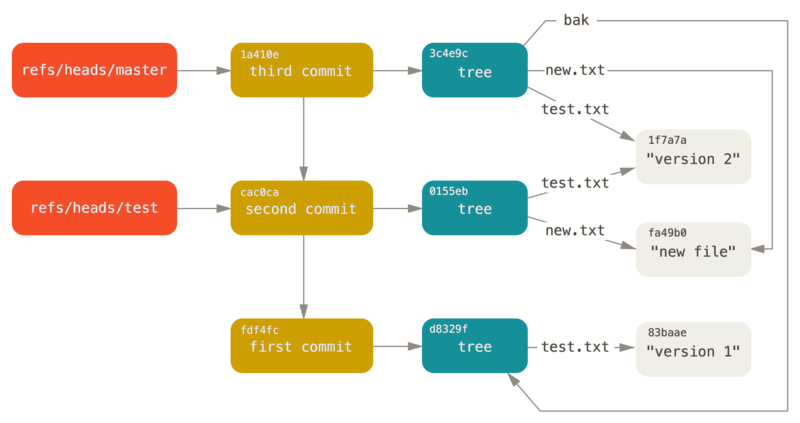
\includegraphics[width=1\textwidth]{git.png}
Dobre wsparcie dla rozgałęzionego procesu tworzenia oprogramowania: jest dostępnych kilka algorytmów łączenia zmian z dwóch gałęzi, a także możliwość dodawania własnych algorytmów.

Praca off-line: każdy programista posiada własną kopię repozytorium, do której może zapisywać zmiany bez połączenia z siecią; następnie zmiany mogą być wymieniane między lokalnymi repozytoriami.

Wsparcie dla istniejących protokołów sieciowych: dane można wymieniać przez HTTP(S), FTP, rsync, SSH.

Efektywna praca z dużymi projektami: system Git według zapewnień Torvaldsa, a także według testów fundacji Mozilla, jest o rzędy wielkości szybszy niż niektóre konkurencyjne rozwiązania.

Każda rewizja to obraz całego projektu: w przeciwieństwie do innych systemów kontroli wersji, Git nie zapamiętuje zmian między kolejnymi rewizjami, lecz kompletne obrazy. Z jednej strony wymaga to nieco więcej pracy aby porównać dwie rewizje, z drugiej jednak pozwala np. na automatyczną obsługę zmian nazw plików.

\newpage
\section{LaTeX}
\subsection{Opis}
LaTeX to zestaw makr zaprojektowany przez Leslie Lamporta stanowiących nadbudowę nad systemem składu tekstu TeX, będącym kompletnym językiem programowania zaimplementowanym przez Donalda Knutha. Jego celem jest umożliwienie stworzenia profesjonalnie wyglądających oraz poprawnie złożonych dokumentów, szczególnie naukowych – zawierających matematyczne wzory – oraz dokumentów działających automatycznie (szablonowo).

LaTeX znacznie różni się od programów typu WYSIWYG (ang. What You See Is What You Get – widzisz to, co dostajesz, m.in. OpenOffice.org Writer lub Microsoft Word) i jego użycie przypomina bardziej programowanie. Do podstawowych trudności dla nowych użytkowników LaTeX-a należą:

składanie dokumentów może sprawiać trudności i zabierać czas niedoświadczonym użytkownikom
nie widać bezpośrednio efektu zmian
musisz poznać niezbędne polecenia w LaTeX-u
czasami ciężko uzyskać pożądane efekty.
Z drugiej strony taki język znaczników posiada także zalety:

dokument wygląda profesjonalnie, m.in. warstwy, fonty, tabele tworzą spójną całość
zachęca do tworzenia poprawnych pod względem struktury dokumentów
profesjonalnie złożone dokumenty charakteryzuje mała objętość w porównaniu do zawartości
w łatwy sposób można tworzyć matematyczne wzory
pozwala na zaawansowaną automatyzację składania dokumentów
indeksy, odwołania i bibliografie mogą być automatycznie formatowane
obsługuje praktycznie każdy komputer i system operacyjny identycznie składając dokumenty na każdym
dokument źródłowy jest plikiem tekstowym, zatem jego wersjonowanie jest możliwe (porównywanie wersji, przypisywanie autora do konkretnej treści/zmian).
Dokument LaTeX-a jest normalnym plikiem tekstowym, który przechowuje tekst z dodatkowymi znacznikami. Kiedy plik źródłowy zostanie przetworzony LaTeX-em otrzymamy plik DVI (ang. device-independent), który potem może zostać przekonwertowany do finalnego formatu np. PDF lub PostScript, które można łatwo wydrukować. Jest również możliwe bezpośrednie utworzenie pliku w formacie PDF.
\newpage

  \begin{thebibliography}{9}

  \bibitem{Model TCP/IP}
  Wikipedia.org
  \textit{Model TCP/IP},
  Społeczeństwo Wikipedia,
 
   \bibitem{SDN}
  Wikipedia.org
  \textit{ sdn},
  Społeczestwo Wikipedia,
  
  \bibitem{python}
  Wikipedia.org
  \textit{ Python},
  Społeczeństwo Wikipedia,
  https://pl.wikipedia.org/wiki/Python
  2002.

  \bibitem{jupyter}
  Wikipedia.org
  \textit{Jupyter - wprowadzenie},
  perseba.github.io,
  http://perseba.github.io/blog/jupyter-wprowadzenie.html
  2015.

  \bibitem{LaTeX}
  Wikibooks.org
  \textit{LaTeX},
  Społeczność Wikibooks,
  https://pl.wikibooks.org/wiki/LaTeX
  2015.


  


\end{thebibliography}
\end{document}
